\section*{Background}

\begin{frame}{Context}
    \begin{itemize}
        \item Path planning episodes are independent;
        \item each episode has fixed start and target locations;
        \item graph map is known a priori.
    \end{itemize}
    
    \medskip
    ``Perturbations'': \footnote{\todo{give definition of perturbations from paper?}}
    \begin{itemize}
        \item[-] distribution over map unknown a priori;
        \item[-] only increase original edge costs;
        \item[-] detected at the beginning of each path planning episode and assumed fixed.
    \end{itemize}
\end{frame}

\begin{frame}{Compressed Path Database (\CPD{})}
    \begin{minipage}{0.33\textwidth}
        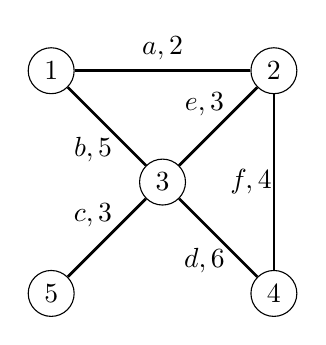
\begin{tikzpicture}
            \tikzset{Vertex/.style={%
                    shape=circle,%
                    draw=black,%
                    minimum size=10pt,%
                    radius=1cm,%
                    inner sep=3pt,%
                    node distance=1.7cm,%
                }}
        
                \node[Vertex] (3) at (0,0) {$3$};
                \node[Vertex] (2) at (+45:2) {$2$};
                \node[Vertex] (1) at (+135:2) {$1$};
                \node[Vertex] (4) at (-45:2) {$4$};
                \node[Vertex] (5) at (-135:2) {$5$};
                
        
                \path (1) edge[-,line width=1pt] node[above]{$a,2$} (2);
                \path (2) edge[-,line width=1pt] node[left,xshift=+3pt]{$f,4$} (4);
                \path (3) edge[-,line width=1pt] node[below,xshift=-5pt]{$b,5$} (1);
                \path (3) edge[-,line width=1pt] node[above,xshift=-5pt]{$e,3$} (2);
                \path (3) edge[-,line width=1pt] node[below,xshift=-5pt]{$d,6$} (4);
                \path (3) edge[-,line width=1pt] node[above,xshift=-5pt]{$c,3$} (5);
        \end{tikzpicture}
    \end{minipage}\hfill%
    \begin{minipage}{0.33\textwidth}
        % see https://tex.stackexchange.com/a/317083/145331
        \begin{table}
            \centering
            \begin{tabular}{l|ccccc}
            \diaghead(5,-3){\theadfont xx}{\hphantom{x}\hphantom{x}t}{s\hphantom{x}\hphantom{x}} 
                & 1 & 2 & 3 & 4 & 5 \\ \hline
                1 & - & $a$ & $a$ & $a$ & $a$ \\
                2 & $a$ & - & $e$ & $f$ & $e$ \\
                3 & $e$ & $e$ & - & $d$ & $c$ \\
                4 & $f$ & $f$ & - & $d$ & $d$ \\
                5 & $c$ & $c$ & $c$ & $c$ & - \\
            \end{tabular}
        \end{table}
    \end{minipage}\hfill%
    \begin{minipage}{0.33\textwidth}
        $$(s,t) = (1, 5)$$
        $$M[1, 5] = a$$
        $$M[2, 5] = e$$
        $$M[3, 5] = c$$
        $$1 \rightarrow 2 \rightarrow 3 \rightarrow 5$$
    \end{minipage}

\end{frame}

\begin{frame}{\ALT{} and Anytime Weighted A* (\AWA{})}
    \textbf{\ALT{}:}
    \begin{itemize}
        \item Search technique using preprocessed \textit{landmarks} to derive admissible
            estimates of every node pair $(s, t)$;
    \end{itemize}
    \textbf{\AWA{}:}
    \begin{itemize}
        \item TODO
    \end{itemize}
\end{frame}